%%
%% This is file `sample-sigconf.tex',
%% generated with the docstrip utility.
%%
%% The original source files were:
%%
%% samples.dtx  (with options: `sigconf')
%% 
%% IMPORTANT NOTICE:
%% 
%% For the copyright see the source file.
%% 
%% Any modified versions of this file must be renamed
%% with new filenames distinct from sample-sigconf.tex.
%% 
%% For distribution of the original source see the terms
%% for copying and modification in the file samples.dtx.
%% 
%% This generated file may be distributed as long as the
%% original source files, as listed above, are part of the
%% same distribution. (The sources need not necessarily be
%% in the same archive or directory.)
%%
%% The first command in your LaTeX source must be the \documentclass command.
\documentclass[sigconf]{acmart}
%% NOTE that a single column version may be required for 
%% submission and peer review. This can be done by changing
%% the \doucmentclass[...]{acmart} in this template to 
%% \documentclass[manuscript,screen]{acmart}
%% 
%% To ensure 100% compatibility, please check the white list of
%% approved LaTeX packages to be used with the Master Article Template at
%% https://www.acm.org/publications/taps/whitelist-of-latex-packages 
%% before creating your document. The white list page provides 
%% information on how to submit additional LaTeX packages for 
%% review and adoption.
%% Fonts used in the template cannot be substituted; margin 
%% adjustments are not allowed.
%%
%%
%% \BibTeX command to typeset BibTeX logo in the docs
\usepackage{caption}
\captionsetup{skip=6pt}
\AtBeginDocument{%
  \providecommand\BibTeX{{%
    \normalfont B\kern-0.5em{\scshape i\kern-0.25em b}\kern-0.8em\TeX}}}

%% Rights management information.  This information is sent to you
%% when you complete the rights form.  These commands have SAMPLE
%% values in them; it is your responsibility as an author to replace
%% the commands and values with those provided to you when you
%% complete the rights form.

\copyrightyear{2021}
\acmYear{2021}
\setcopyright{acmcopyright}
\acmConference[K-CAP '21] {Proceedings of the 11th Knowledge Capture Conference}{December 2--3, 2021}{Virtual Event, USA.}
\acmBooktitle{Proceedings of the 11th Knowledge Capture Conference (K-CAP '21), December 2--3, 2021, Virtual Event, USA}
\acmPrice{15.00}
\acmISBN{978-1-4503-8457-5/21/12}
\acmDOI{10.1145/3460210.3493579}
% Authors, replace the red X's with your assigned DOI string during the rightsreview eform process.



%%
%% Submission ID.
%% Use this when submitting an article to a sponsored event. You'll
%% receive a unique submission ID from the organizers
%% of the event, and this ID should be used as the parameter to this command.
%%\acmSubmissionID{123-A56-BU3}

%%
%% The majority of ACM publications use numbered citations and
%% references.  The command \citestyle{authoryear} switches to the
%% "author year" style.
%%
%% If you are preparing content for an event
%% sponsored by ACM SIGGRAPH, you must use the "author year" style of
%% citations and references.
%% Uncommenting
%% the next command will enable that style.
%%\citestyle{acmauthoryear}

%%
%% end of the preamble, start of the body of the document source.
\settopmatter{printacmref=true}
\begin{document}
\fancyhead{}
%%
%% The "title" command has an optional parameter,
%% allowing the author to define a "short title" to be used in page headers.
\title{Knowledge Engineering of PhD Stories: A Preliminary Study}

%%
%% The "author" command and its associated commands are used to define
%% the authors and their affiliations.
%% Of note is the shared affiliation of the first two authors, and the
%% "authornote" and "authornotemark" commands
%% used to denote shared contribution to the research.
\author{Viet Bach Nguyen}
%\authornote{Both authors contributed equally to this research.}
\email{viet.nguyen@vse.cz}
\orcid{0000-0003-2709-3297}
\author{Vojtech Svatek}
%\authornotemark[1]
\email{svatek@vse.cz}
\orcid{0000-0002-2256-2982}
\author{Marek Dudas}
\email{marek.dudas@vse.cz}
\orcid{0000-0002-9388-8322}
\affiliation{%
  \institution{Prague University of Economics and Business}
  \streetaddress{W. Churchill sq. 1938/4}
  \city{Prague}
  \country{Czech Republic}
}

\author{Oscar Corcho}
\orcid{0000-0002-9260-0753}
\affiliation{%
  \institution{Universidad Politecnica de Madrid}
  \streetaddress{Campus de Montegancedo, sn}
  \city{Madrid}
  \country{Spain}
}
\email{ocorcho@fi.upm.es}

%%
%% By default, the full list of authors will be used in the page
%% headers. Often, this list is too long, and will overlap
%% other information printed in the page headers. This command allows
%% the author to define a more concise list
%% of authors' names for this purpose.
\renewcommand{\shortauthors}{Nguyen, et al.}
 
%%
%% The abstract is a short summary of the work to be presented in the
%% article.
\begin{abstract}
Support for PhD students and their advisors in decision-making before and along their PhD journeys requires providing them with a deep understanding and knowledge of the life-cycle of a PhD. This means giving them access to a thorough understanding of causal relations between events, decisions, and the possible outcome. This knowledge can be attained primarily from insider stories, study reports, communications threads with advisors and colleagues, interviews, and scholarly databases. However, it is unclear how to give this knowledge a reasonable structure (due to the heterogeneity of concepts and data sources) so that we can use it for decision-making during the PhD journey. In this paper, we explore how to analyze and model PhD stories to uncover and extract causal relationships found within each story to get insights into the co-occurrences and causalities. We analyze these stories with thematic analysis to understand their main points and we use concept maps to create semi-formal graphs of connected events and objects where the relationships are being emphasized from the perspective of cause and effect. Our results at this point are a collection of PhD stories in the form of concept maps, thematic codes, a proposed approach for goal-directed PhD story modeling which we describe in this paper.
%methodology,  
%a catalog of (quasi)causalities, 
%and the lessons learned from modeling these stories.
\end{abstract}

%%
%% The code below is generated by the tool at http://dl.acm.org/ccs.cfm.
%% Please copy and paste the code instead of the example below.
%%
\begin{CCSXML}
<ccs2012>
    <concept>
        <concept_id>10002944.10011122.10002948</concept_id>
        <concept_desc>General and reference~Biographies</concept_desc>
        <concept_significance>500</concept_significance>
    </concept>
    <concept>
        <concept_id>10003752.10010124</concept_id>
        <concept_desc>Theory of computation~Semantics and reasoning</concept_desc>
        <concept_significance>500</concept_significance>
    </concept>
</ccs2012>
\end{CCSXML}

\ccsdesc[500]{General and reference~Biographies}
\ccsdesc[500]{Theory of computation~Semantics and reasoning}
%\ccsdesc{Computer systems organization~Robotics}
%\ccsdesc[100]{Networks~Network reliability}

%%
%% Keywords. The author(s) should pick words that accurately describe
%% the work being presented. Separate the keywords with commas.
\keywords{causal relation, causality, concept map, knowledge engineering, PhD story modeling, thematic analysis}

%% A "teaser" image appears between the author and affiliation
%% information and the body of the document, and typically spans the
%% page.
%\begin{teaserfigure}
%  \includegraphics[width=\textwidth]{sampleteaser}
%  \caption{Seattle Mariners at Spring Training, 2010.}
%  \Description{Enjoying the baseball game from the third-base
%  seats. Ichiro Suzuki preparing to bat.}
%  \label{fig:teaser}
%\end{teaserfigure}

%%
%% This command processes the author and affiliation and title
%% information and builds the first part of the formatted document.
\maketitle

\section{Introduction}
A PhD journey is a long-term process
%a long-term and unique starting process 
of a scholar learning how to conduct research and advance in a research area.
%pursuing knowledge and answers to research problems. 
Each PhD journey is a unique experience consisting of several %main 
stages depending on the study program. Throughout each PhD journey, many decisions are made and many events happen that lead to a (un)favorable outcome. It is, however, a pity that almost 50\% of doctoral students do not graduate \cite{councilofgraduateschools}, which also affects the overall PhD research quality in the world. To provide better support and improve %the 
PhD research quality and study retention, it is necessary to gather insights into the co-occurrences and causalities in PhD stories and structure the information, e.g., in a knowledge graph, for practical use. This knowledge base populated with entities from the stories would be analyzed to discover recurrent patterns. These patterns would be kept as an additional layer of the knowledge base, and divided to best practice (what should be followed), anti-pattern (what should be avoided), and neutral. In this context, the most profiting users would be the advisors or PhD program managers, who could better understand the issues in the PhD domain. Top-level focus questions guiding the choice of concepts in a PhD story would be possible reasons and drivers for the eventual success or failure and achieving good research results. The main use cases for such a system would be to inform and educate prospective PhD applicants and to support on-going PhD students and their advisors using the discovered patterns and the inference over them. This envisioned system would consist of a knowledge base with search functionalities and a serious game built on top of it, as well as an interface for users to model and annotate their own stories.
%\begin{itemize}
%    \item possible reasons for the eventual success or failure,
%    \item possible reasons for achieving good research results.
%\end{itemize}

To effectively understand the PhD story passage, it is essential to emphasize the causal relationship between events and decisions. In this paper, we begin exploring the possibility of capturing and analyzing PhD stories to extract events and causal relationships from them using thematic analysis coding method \cite{thematic_analysis} and concept maps. %In the scope of this paper, 
We mainly focus on stories from the research field of \textit{Applied Informatics} and have gathered several PhD stories from various types of sources like evaluation reports, %CVs, 
blog posts, and interviews %notes and emails of PhD advisors
for analysis. Our goal is to create semi-structured graphs of events that are important for individual PhD stories and annotate them with abstract concepts. These graphs could then be selectively enriched from structured knowledge graphs with, e.g., data about publications. The result so far is a collection of modeled PhD stories in the form of concept maps, thematic codes from stories, and a proposed PhD story modeling approach based on exploratory experiments. %, and the lessons learned from modeling these stories that can outline findings useful for analyzing causal links within events. % to develop computer-based simulations and teach students on decision-making.

\section{Related work}
\label{section:related-work}
We are unaware of any project having the same target and similar technology as ours. 
%R1
However, PhD stories themselves have indeed been studied, but using social science, rather than knowledge engineering techniques.
%R2
%Moreover, 
PhD stories as subjects of knowledge modeling have several features shared with slightly different targets addressed in prior research. 
%R3 
Also, the story itself bears some similarities to a scientific workflow. 
%R4
On the other hand, being a story of a particular person, it can be viewed as a special kind of partial biography. 
%R5
Furthermore, as the purpose of the story modeling is the capturing of causality, we could align them to causal ontologies. 
%R6
And, in the field of EduTech, serious games are used to train students in higher education to better get acquainted and improve performance.

\medskip
\noindent \textbf{Social science}.
%XR1
Studies on PhD journeys have been active in the social science field commonly based on ethnographic studies. % as well. 
We have stumbled upon some projects that directly address the issues in the PhD life and show the significance of the amount of workload and the relationship between advisors and PhD students \cite{doi:10.1080/0158037X.2019.1652158}.%, also how to identify the needs to help and support the well-being and academic functioning of PhD students by leveraging brief mindfulness-based intervention therapies \cite{Kaczan2015ItsA}, and a predictive model of dropout intentions \cite{LITALIEN2015218}.

\medskip
\noindent \textbf{Knowledge modeling}.
%XR2
In our prior work \cite{DBLP:conf/ekaw/NguyenSRC20}, we addressed knowledge patterns used by researchers during information foraging, in specific contexts. Unlike our current project, the patterns only involved entity links that are accessible through public resources, and the considered target was that of satisfying a fine-grained information need rather than of undertaking a complex research activity such as a PhD project.

\medskip
\noindent \textbf{Scientific workflows}.
%XR3
Knowledge graphs and ontologies have been a strong focus for research in the Semantic Web field in recent years, namely in the scholarly, researcher, and academic domains. 
A systematic and provenance- and ontology-based approach is used for semantically explaining conducted scientific experiments with the primary goal of reproducibility by describing the whole story path of these experiments \cite{samuelsheeba}. %It is clear that
The primary focus of this project is set on the level of individual research experiments, which can be perceived as a component of the whole PhD journey as they are much more detailed with a focus on projects, rather than on an individual researcher, whose PhD journey may encompass several interrelated projects and numerous experiments. Our modeling of PhD stories primarily aims at extracting and aggregating patterns; even if a real story were taken as an example to be \textit{reproduced}, this reproduction occurs at a rather approximate level. There are, however, entities likely to appear in both kinds of models, e.g., collaborator, artifacts, datasets, tools, experiments, etc.

\medskip
\noindent \textbf{Biography}.
%XR4
Further relevant state-of-the-art projects involving knowledge graphs include the capturing of biographies via systematic knowledge graph building efforts with a social-science flavor \cite{riechert2010} \cite{hyvonen2018}. 
%, e.g., the Catalogus Professorum Lipsiensis \cite{riechert2010} and the Finnish BiographySampo \cite{hyvonen2018}. 
Generally, aspects of biographies are present in common encyclopedic knowledge graphs such as Wikidata and DBpedia, specialized knowledge graphs from publications, or integrative knowledge graphs wrt. the scholarly domain, especially the Open Research Knowledge Graph (ORKG) \cite{DBLP:conf/kcap/JaradehOFPDKSA19}. In the knowledge graph-based approaches, the biographical information is captured at the level of basic CV facts such as birth, marriage, and university degree enrollment/completion, primarily for important historical persons with sufficient digital imprint (even if reconstructed from historical documents). The common encyclopedic and specialized knowledge graphs provide access to biographical data of ordinary and still living researchers, but with an even smaller repertory of biographical detail types, and rather exhaustively while not considering the varying degree of importance. Therefore, both these approaches understandably ignore fine-grained events %(sometimes with no, or siloed, digital imprint) 
that can only be reliably captured by insiders, never mind possible causalities among them. 


\medskip
\noindent \textbf{Causal ontologies}.
%XR5
In the ontology engineering world, causality as a topic has appeared mostly in projects that involve medical and healthcare-related studies \cite{DBLP:conf/ichi/YinPHTCSH20} to capture relationships between diseases and symptoms as well as medical procedures and treatments for, e.g., improving decision support in domain knowledge-based diagnosis \cite{Hong2021}. \cite{DBLP:conf/compsac/HuK20}. 
Other domains of interest are, e.g., construction \cite{9440633}, 
%variant design \cite{10.1115/1.4048127}, 
NLP \cite{9375954}, and fact-checking \cite{doi:10.1061/(ASCE)LA.1943-4170.0000489}. %Causality or 
Causation as a general ontological concept has also been created in ontologies such as DTO \cite{HamdanAl-Hakam2019Aomf}, XKOS \cite{DBLP:conf/semweb/GillmanCJ13}, and BioTop \cite{DBLP:journals/ao/BeisswangerSSH08}. Still, the causal aspect of knowledge capturing for the scholarly domain has not been addressed. A theory of modeling causality on the conceptual level has been, however, summarized in related work \cite{DBLP:conf/jowo/Mizoguchi20}, but no formalization has been proposed as of yet. By modeling the PhD stories in a concept-map manner, we can explore the possibilities of finding sample instance data for causal relationships in the scholarly domain.



\medskip
\noindent \textbf{EduTech and serious games}.
%XR5
In practice, efforts in improving the study retention can be observed in EduTech, where serious games are being applied in higher education \cite{ince}. These games are usually created based on several serious game models and frameworks that provide the appropriate and necessary incentives for users and evaluative measurement techniques.

\section{Research methodology, PhD story collection, analysis and modeling}
%We are interested in 
Our %research methodology 
approach for tackling this research problem consists of several steps, see Fig. \ref{fig:methodology}: literature survey, data source type identification, data collection, story analysis, story modeling, pattern extraction, and understanding causal relationships. 

\begin{figure}[ht]
  \centering
  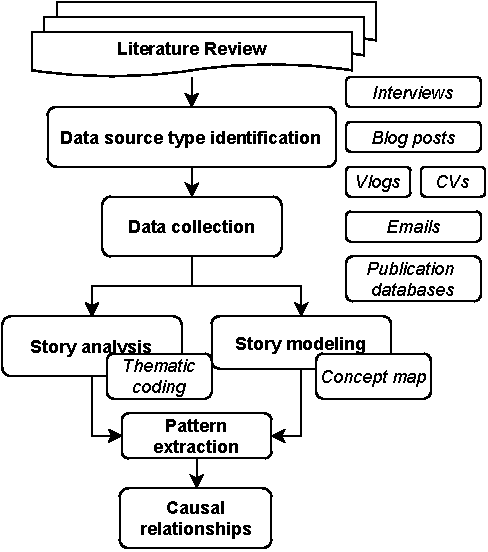
\includegraphics[width=5.9cm]{pictures/methodology.pdf}
  \caption[methodology]{Methodology outline}% for PhD story analysis and modeling}
  \label{fig:methodology}
\end{figure}

First, we looked in the recent literature for similar projects featuring topics of our interest, e.g., PhD story, story modeling, biography, causality in ontology engineering. As mentioned in Section \ref{section:related-work}, we are unaware of any project that focuses on analyzing the PhD narrative to extract causal knowledge for a systematic support solution. %Only projects with similar individual features. 

For identifying data source types, we have consulted with PhD program advisors and PhD alumni and asked them what kind of information is crucial in their stories and in what way they could be retrieved. The undeniable resources are documented stories in various forms, most often blog posts and video logs. Personal information and major turning points could be obtained from CVs, study information systems, and official study records like annual PhD reports. We also learned that the less accessible, but retrievable, resources are communication threads in the form of emails and personal notes of the participants. Last but not least, also a very promising type of resource, are interviews which we conducted with the help of several PhD students in the Applied Informatics field. The variety of data sources already suggests that the necessary information is very scattered, which is difficult to handle.

In the data collection step, we focused on four main sources: PhD advisors, interviews, publication databases, and documented stories on the web.%, see Fig. \ref{fig:data-collection}. 
Since the central subject in each story is the PhD student, we first created a list of candidate names and tried to get as much information as possible through the four mentioned sources for each of them. To extend our collection, we searched over the internet for interesting stories containing good narratives. %At this point we do not know which information is more important than the other, so we considered all of them to be primary. 

%\begin{figure}[ht]
%  \centering
%  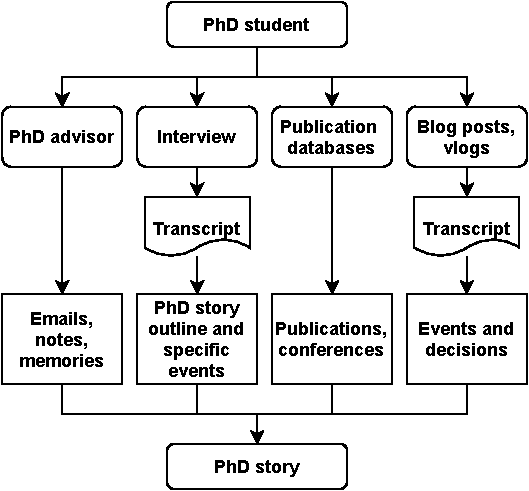
\includegraphics[width=6cm]{pictures/data-collection.pdf}
%  \caption[data-collection]{Data collection}
%  \label{fig:data-collection}
%\end{figure}

This way, we have collected a total of 12 stories, 8 in the form of blog posts and videos, 4 in the form of interviews. We then supplied additional data from emails, annual evaluation reports, and notes of the PhD advisors. Thematic analysis was applied on all stories and concept maps were created for 5 stories.\footnote{
\url{https://app.contextminds.com/?m=L2J7e}, 
\url{https://app.contextminds.com/?m=1nW6E}, 
\url{https://app.contextminds.com/?m=d0wgg}, 
\url{https://app.contextminds.com/?m=NJb7g}, 
\url{https://app.contextminds.com/?m=YBE7j}
}

% We have created several criteria for collecting PhD stories. The stories need to be event-centric, because ...

With the collected data, we proceeded with analyzing and modeling the stories using a proposed method shown in Fig.\ref{fig:story-modeling}. For the analysis part, we used thematic coding technique to find the main points (codes and themes) of the stories. % when they are available as a knowledge-rich text such as an interview or a PhD story blog post. 
For the modeling part, we rely on concept maps where the story is modeled by a story insider. %(PhD advisor, PhD student, and interviewer). %Essentially, 
Both approaches are used partly in parallel and inform one another.

\begin{figure}[ht]
  \centering
  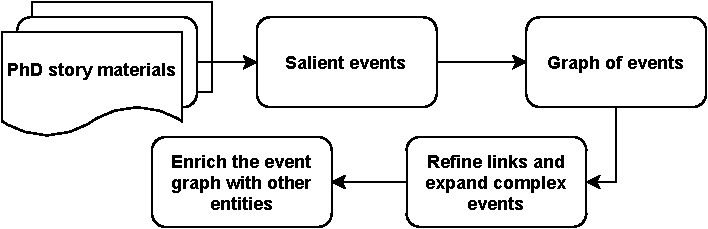
\includegraphics[width=7cm]{pictures/story-modeling.pdf}
  \caption[story-modeling]{PhD story modeling}
  \label{fig:story-modeling}
\end{figure}

During this stage, we have distinguished three main strategies for analyzing a PhD story: 1) \textit{timeline view} -- systematically going through the events in their chronological order; 2) \textit{goal-directed} -- going rather backward, from the completed and successfully defended thesis, or from the point of failure, to the potentially causing events; and 3) \textit{personal impressions} -- going from salient impressions of the student in the given moment, typically based on an interview, and building a cluster of events. These three strategies are described in separate documents listed in our GitHub repository. These approaches provide a solution for how to collect the knowledge from stories with the main goal of providing decision support based on typical causal links that can be used to structure the knowledge.

Our first attempt was based on the timeline view, chronologically going through a story mostly based on annual evaluation reports and publication databases. This led to a richly structured graph with ontology-based flavor, covering entities of many different types residing around the story. Inevitably, the size of the graph grew considerably, which made it hard to manage (even for just two initial years of the story). 
%
The second attempt for a different story involved looking at the thesis and final evaluation reports and matching them with the goals and critical factor model consisting of formal requirements for obtaining the PhD title, and then chronologically going through the story, this time using an available detailed story blog post, but only selecting the salient events, primarily in reference to the filled template of critical factors. This produced a graph of only events, including tentative causalities. 
%
For the third attempt, we tried to include in the model as much information as possible from the stories while connecting events and decisions with ad-hoc links to preserve the narration details.

%Concept maps are nowadays a popular vehicle that allows people to structure their ideas and conceptualization of a domain; used in education, creative copy-writing, management communication, etc. 
We came to the preliminary %methodological 
conclusion that the backbone of each story should be the big and important, salient events throughout a PhD journey. Therefore, the events on the highest conceptual level for the PhD story modeling should correspond to the PhD program passage, such as PhD enrollment, completing subjects of the PhD program, doing internships, research projects, publishing papers, attending conferences, completing state exams, thesis defense. 

We looked at the final or most up-to-date PhD materials like theses, reviews, late-stage evaluation reports, etc., and characterize the ways of satisfying the goals and effect of conditions during the study. %, in a form-filling manner. 
Next, we went through the story chronology (in a PhD blog, e-mail threads, series and evaluation reports, etc.) and annotate the \textit{salient events} in it while using the findings and additional materials (interviews, if available) to judge the salience. The annotated story was used to build a graph of events linked by broadly understood \textit{led to} links, plus some auxiliary ones, e.g. \textit{part of}. The next step was to refine the links and expand complex events to chains. The last step was to enrich the event graph with other entities primarily such that relate to more than one event, e.g., people, projects, conferences, experiments, artifacts, etc. because parts of the stories could be populated from existing knowledge graphs, especially those of publications and their authors.

For modeling stories, %with events leading to other events, 
we used ContextMinds web app\footnote{\url{https://www.contextminds.com}} which allows for lightweight graphical modeling and the possibility of subsequent export of the whole graph to RDF. While the modeling is lightweight compared to knowledge graphs, which are tightly associated with formal ontologies, it is still possible to transform the models (maps) to a formal (RDF) representation relatively easily. The starting point is the concrete stories rather than the domain as such. Thus, the concepts will primarily be ontological particulars while the ontological classes can be approximated via tags, e.g., event, creative work, researcher, experiment, organization, etc.\footnote{\url{https://app.contextminds.com/?m=4K7Ml}}.

%, see Fig. \ref{fig:meta-model}.

The analytical part of our research primarily involves
%a qualitative analysis technique called thematic coding or
%which allows us to understand the story main-points and obtain semi-structured graphs of events.
thematic analysis, a relatively lightweight qualitative research method frequently applied on knowledge-rich texts such as interviews. This technique suggests highlighting sections of transcripts and textual materials with \textit{codes} to describe the content by going through and highlighting everything that we selectively perceive as relevant to our questions or potentially interesting from the story. The data are then grouped using these codes which allows us to gain a condensed overview of the main points %and common meanings 
that recur throughout the data. Codes are then reviewed and combined to identify \textit{themes} or \textit{types} that help us understand the meaning of the content and identify concepts and terms in the domain of interest. Our primary goal for analyzing PhD stories using this method is to provide ideas for tags and concepts to be then suggested in graphical modeling. % via patterns. 
The most significant result of this analysis is a list of keywords and their types found in the stories, see Tab. \ref{table:thematic-coding}.%, which could serve as a dictionary of domain terms.

\begin{table}[ht]
\small
\caption[coding results]{Thematic coding results examples\footnotemark}
\label{table:thematic-coding}
\begin{tabular}{|l|l|l|l|l|}
\hline
\multicolumn{5}{|l|}{\textbf{Codes}}                                                   \\ \hline
Term              & Teaching               & Paper        & Advisor       & Experiment \\ \hline
Journal           & Meeting                & Survey       & Consultation  & ...        \\ \hline
%...               & ...                    & ...          & ...          & ...        \\ \hline 
\hline
\multicolumn{5}{|l|}{\textbf{Types}}                                                   \\ \hline
Achievement       & Document               & Event        & Institution   & ...        \\ \hline
%...               & ...                    & ...          & ...          & ...        \\ \hline
\end{tabular}
\end{table}
\footnotetext{Full table: \url{https://github.com/nvbach91/phd-odyssey/tree/master/thematic-analysis}}

%\begin{figure*}[ht]
%  \centering
%  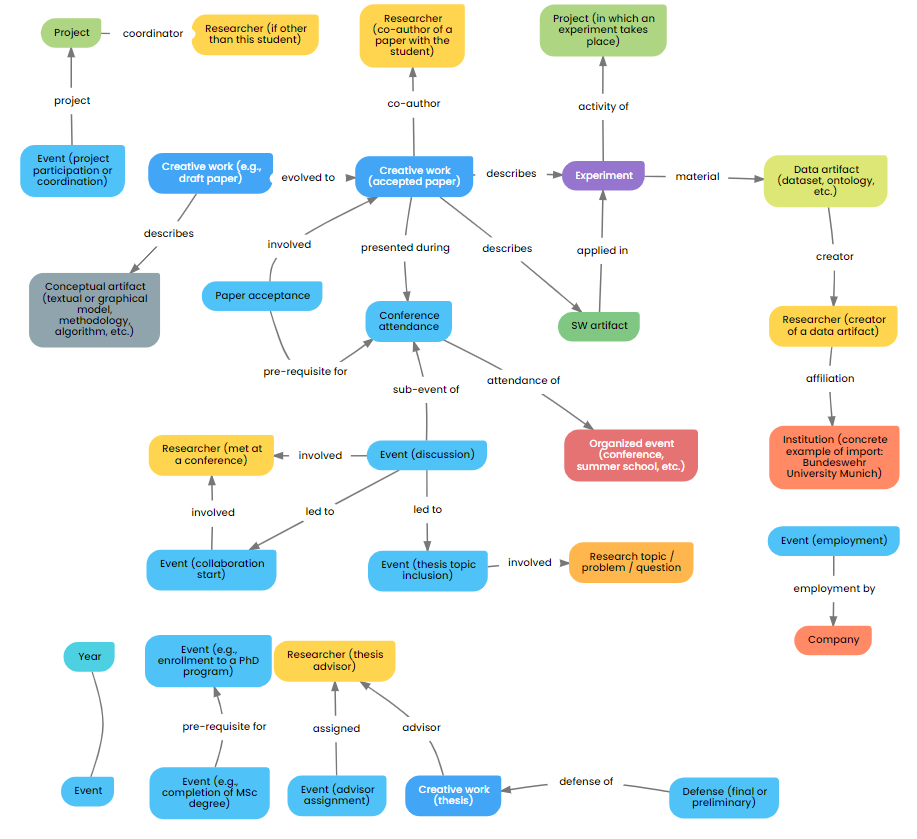
\includegraphics[width=\textwidth]{pictures/meta-model.png}
%  \caption{Meta-model for PhD stories}
%  \label{fig:meta-model}
%\end{figure*}

%\caption{Thematic analysis -- coding results}


%\section{Evaluation?}
%We gave it to the PhD alumni themselves and see if they had something to add?

\section{Conclusion and future work}
In this paper, we have presented our first effort towards exploring and creating a method for collecting, analysis and modeling of PhD stories in order to give structure to the knowledge found within them, which we hope will be useful in the development of a knowledge-based information system that can provide knowledge support for PhD students and their advisors. After literature review and identifying data source types, we have used thematic coding and the proposed story modeling approach to analyze the collected data and build PhD stories in the forms of concept maps. The results of this preliminary study are published on GitHub\footnote{\url{https://github.com/nvbach91/phd-odyssey}} including analyzed stories, coding results, and modeled stories.
%We used thematic coding method and concept maps to explore and model the stories. 

%we have created a preliminary meta model for modeling PhD stories and a goal-directed PhD story modeling methodology, a catalog of (quasi)causalities. Furthermore, we have distilled a list of lessons learned from modeling these stories as to outline the findings of causal links within events. 
The proposed approach has limitations: the stories analysis and modeling are not easily replicated as all steps must be repeated for new stories, apart from thematic coding, where codes can be reused. We intend to apply crowd-sourcing by the PhD students and graduates themselves for the approach to scale. For this, we would presumably need a dedicated story editor or annotator for submitting stories in a semi-structured form. 
%These could be improved in the next iteration by: ... which will allow us to better ...

Future work will include creating a system for capturing stories as concept maps by stakeholders (students, graduates, and advisors), and adding support for pre-population of concept maps from existing resources like structured knowledge graphs. %, eventually via text mining from PhD blogs as a secondary source of data. 
We also intend to bring in an extensive usage of a concept reuse functionality in ContextMinds to allow to cluster the stories. We plan to conduct a systematic use of qualitative research methods to build an insightful model that would guide further quantitative experiments and rule mining from co-occurrences of events in PhD stories. Lastly, we plan to prepare a requirement analysis for a knowledge-based search application over PhD concepts and a serious game that simulate the course of the study (primarily for early-phase students and people considering the pros and cons of enrolling to a PhD program in Applied Informatics).
%%
%% The acknowledgments section is defined using the "acks" environment
%% (and NOT an unnumbered section). This ensures the proper
%% identification of the section in the article metadata, and the
%% consistent spelling of the heading.
\begin{acks}
This research was supported by the project IGA V\v{S}E \textnumero\ F4/56/2021.
\end{acks}
%\medskip
%\noindent \textbf{Acknowledgement}. This research was supported by project IGA V\v{S}E \textnumero\ %F4/56/2021.

%%
%% The next two lines define the bibliography style to be used, and
%% the bibliography file.
\bibliographystyle{ACM-Reference-Format}
\bibliography{references}


\end{document} 
\endinput
%%
%% End of file `sample-sigconf.tex'.
